\chapter{GraphDB}
\chapterauthor{Thore Krüss, Lennart Purucker, Johanna Sommer}

\section{Motivation/Introduction}
First paragraph to state the general context and make important points for the motivation and why its important. Refer to Wood Paper here.

But Graph Database research has its beginnings already in the early 90s. During this time, numerous proposals came up, describing a semantic network to store data about the database. That was, because contemporary systems were failing to take into account the semantics of a database. (letzten Satz ändern)
The Locial Data Model \cite{KUPERLDM} was proposed, trying to combine the advantages of relational, hierarchical and network approaches in that they modeled databases as directed graphs, with leaves representing attributes and internal nodes posing as connections between the data. \\
Similar to that, the Functional Data Model \cite{Shipman1979} was proposed with the same goal, focusing specifically on providing a conceptually natural database interface \cite{Angles2018AnIT}. \\
During this period, most of the underlying theory of Graph Databases was created.
It was most likely because of insufficient hardware support for big graphs that this research declined, only to be picked up again now, powered by improved hardware. Todays focus in Graph Theory research lies primarily on actual practical systems and on the theoretical analysis of graph query languages \cite{Angles2018AnIT}.

Especially practical implementations of Graph Database Theory have gained traction, as real world problems are more often than not interrelated - hence graphs are extremely useful in unterstanding the wide diversity of real-world datasets.\cite{Robinson2013} \\
The emerging of social networks have naturally helped graph database models come up, with big players like Twitter and their implementation FlockDB entering the field. In those social network situations, a so-called social graph can effortlessly model attributes of a person as well as relationships between people. While in traditional RDBMS the apparent friend-of-a-friend-problem would be solved with a join over all relevant tables, in graph database technology this can be achieved with a traversal, which is far more cost inexpensive (letzten Teilsatz ändern) \cite{Miller2013GraphDA}. \\
Another meaningful topic today are recommender systems, where most work focusing on optimizing machine learning algorithms. But also in database theory, this specific context poses challenges. However again, the graph model gracefully maps item similarities and correlations between user behaviour \cite{Huang2002}.

These application fields bring very distinct workloads that require specific query languages to process. There are two different kinds of workload: in social network transactions low-latency online graphs are processed while for example link analysis algorithms evaluate high-throughput offline graphs \cite{Angles2018AnIT}. Many query language proposals have come up recently, differing mainly in the underlying graph data structure/model and the functionality provided \cite{Wood2012QueryLF}.

A deeper description of the theory behind graph databases will be given in subsection 2, aiming to connect the data model to its fields of application as well as comparing it to RDBMS. This comparison will be picked up in subsection 3, where a use case from the SQL world will be applied to Graph Database Theory, focusing in particular on Neo4j. Lastly, our findings will be stated in subsection 4 with a general conclusion.


\section{Graph Database Theory}
\subsection{Description of data model and functionality}
\subsection{fields of application}
\subsection{CAP Theorem}
\subsection{Comparison: Graph Databases and Relational Databases}
As the comparison between Graph Databases and Relational Databases is a known field, a lot of literature exists on this topic already. Throughout the comparisons, the two methods are always assessed under the same aspects: performance, flexibility, security and maturity. \\
For those comparison points it makes sense to focus on specific implementations of the technologies, hence in this section Neo4j will be chosen as a concrete precedent for Graph Databases, whereas MySQL will be the example implementation for Relational Databases.

\subsubsection{Performance}
Detailed surveys on performance of both technologies already exist in literature, for example from Vicknais et al. \cite{Vicknair2010}. In this specific instance, MySQL version 5.1.42 and Neo4j-b11 were compared.
The queries chosen for the experiments were similar to types that are used in real world provenance systems. Typically in this scenario, for one dataset/node one traverses the graph to find its origin. Another use case in this context is, if a data object or node is deemed incorrect, this information needs to be propagated to all its descendants/child nodes \cite{Vicknair2010}.\\
Further on, the queries were partitioned into structural queries referencing the graph but not the payload itsself, and data queries using the actual payload data. It is important to note that the payload data in this case was integer payload data, as different types are handled seperately depending on framework.\\
In the traversal queries, Neo4j clearly outperformed MySQL, sometimes even being faster by the factor of 10. Though that was expected, as Relational Databases are not designed for traversals. MySQL for this part of experiment falls back to a standard Breath First Search, which is not optimal for this scenario. Neo4j on the other hand has a built in framework for traversals, making it superior in terms of performance for the traversal queries \cite{Vicknair2010}. \\
Contrary to that, in the data queries MySQL turned out to be more efficient. This result was partly due to the fact that Neo4j uses Lucene for querying, which treats all payload as text, eventhough in this scenario the payload is of type integer. But also when the payload changes to text, MySQL had better performance in the experiments \cite{Vicknair2010}. \\
The researchers also took into account a special case for the experiments, trying the data queries with payload that is closer to actual real world data - text with spaces inbetween the words. Surprisingly, at a large enough scale Nao4j outperformed MySQL by a large amount for those queries.

\subsubsection{Flexibility}
The flexibility aspect compares both database technologies in their behaviour when taken out of the environment that they were created for \cite{Vicknair2010}. \\
For Relational Databases an uncommon environment would for example be ad-hoc data schemes that change with time, whereas for Graph Databases a less typical dataset would be one without many connections between the individual nodes  \cite{GarimaAnalysis}.
MySQL is optimized for a large-scale multi-user environment, hence trying to use it for smaller applications comes with a large overhead of functionality that has to be implemented with it but that may not even be needed for this specific application.
Neo4j is typically targeted towards more lightweight applications, but manages to scale really well, having a scalable architecture that also accounts for speed \cite{neo4jweb}. Its easily mutable schema makes it more flexible with data types that are rather untypical for Graph Databases.

\subsubsection{Security}
Neo4j does not have built in mechanisms for managing security restrictions and multiple users \cite{GarimaAnalysis}. MySQL on the other hand natively supports multiple users as well as access control lists. \cite{mysqlsecurity}

\subsubsection{Maturity}
For the comparison under the aspect of maturity it makes sense to talk about database implementations in general. Maturity refers both to how old a particular system is and to how thoroughly tested it is \cite{Vicknair2010}.
Since all Relational databases - inclusing MySQL - use the same query language SQL, support is equal over all implementations and support for one implementation is applicable to all others \cite{GarimaAnalysis}.
Neo4js version 1.1 was released in February 2010. While Neo4j is a for-profit framework and has decent support from its parenty company, this does not apply to all graph database implementations \cite{Vicknair2010}. Furthermore, the query languages differ from implementation to implementation, separating them in that aspect and not sharing support??.

\section{Implementation with Neo4j}
In this section the general setup of Neo4j should be lined out and a sample project be described utilizing available Python-Libraries to implement a sample use case.

\subsection{Use Case from the SQL world}

\subsection{Installation}

\subsection{Modelling}
\subsubsection{General Conzept of a Database Model}
There are a couple of guides available describing how to build a database model for Neo4j. Since the database itself is schema-less multiple schmeas can be built and implemented at the same time.
Nevertheless an application needs a model of the data.
Neo4j states in \autocite{neo4j:rel_to_graph} that it is possible to transfer almost all existing relational models into a graph model.
The general approach has been described in \autocite{dzone:rel_to_graph}.
To convert a relational model into a graph tables should be considered as labels.
Foreign keys should be removed and be converted to relations.
JOIN-Tables become relations with additional properties \autocite{neo4j:graph_vs_rdbms}.
The remaining rows will be converted into nodes connected by edges based on the formerly converted relations.

\subsubsection{Implementation of a database model}
While it is possible to manage the database utilizing the CRUD-functionality from Cypher (see \ref{sec:graphdb:cypher}) this is not really comfortable in an application.
Developers familiar with Object-Relational-Mappers (ORM) such as Hibernate for Java or SQLAlchemy for Python would prefer to define the different nodes and relations in common objects.
For Python there is such an Object-Graph-Mapper (OGM) -- neomodel, which is a community driven project to integrate Neo4j into a Python application, published under MIT-License.

The database model in \ref{lst:graphdb:neomodel} has been built following the neomodel documentation \autocite{neomodel:rtd} describing a relatively simple database structure.
This database maps the relations in a social network.
As it can be seen in \ref{fig:graphdb:graphmodel} there may be an arbitrary number of Persons (orange) who may be friends with other persons.
Additionally they can share interests (green) and may be a member of a group (purple).
Forthermore they can state from which country (yellow) they are from.

\begin{figure}[ht]
    \centering
    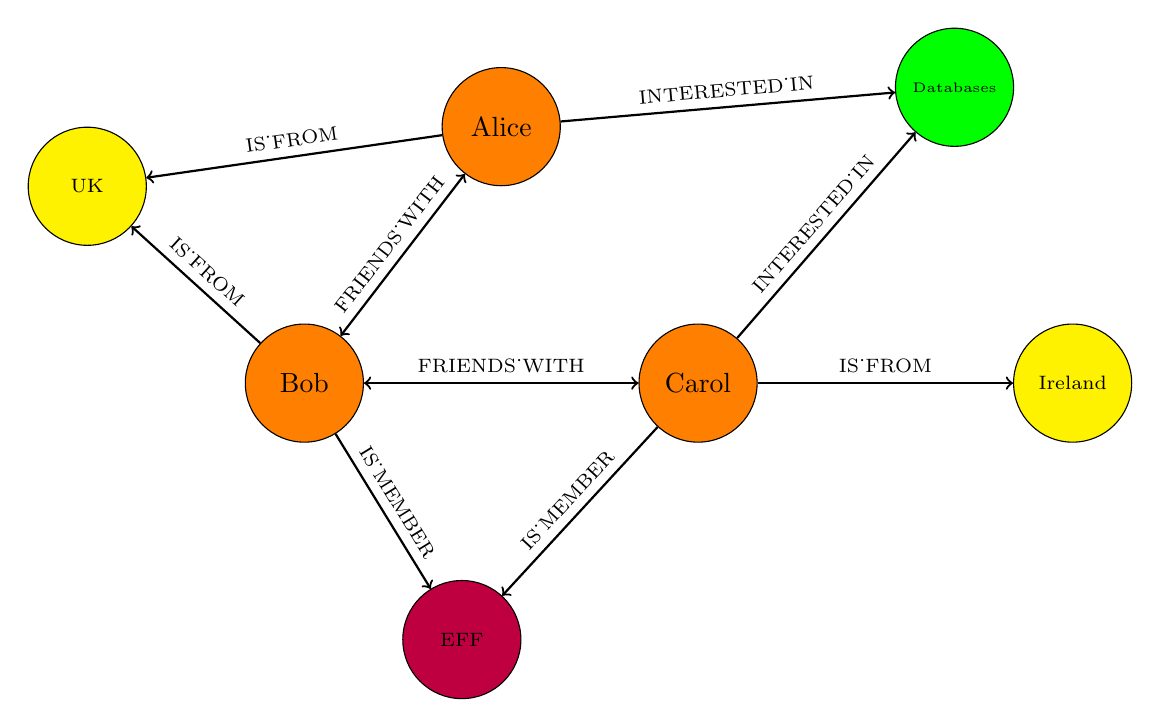
\begin{tikzpicture}
        \node[draw, circle, fill=orange, minimum height=1.5cm, minimum width=1.5cm] (alice) {Alice};
        \node[draw, circle, fill=orange, minimum height=1.5cm, minimum width=1.5cm] (bob)  at ([xshift=-2.5cm, yshift=-2.5cm]alice.south) {Bob};
        \node[draw, circle, fill=orange, minimum height=1.5cm, minimum width=1.5cm] (carol)  at ([xshift=2.5cm, yshift=-2.5cm]alice.south) {Carol};

        \node[draw, circle, fill=green, minimum height=1.5cm, minimum width=1.5cm] (db) at ([xshift=5cm, yshift=0.5cm]alice.east) {\tiny Databases};

        \node[draw, circle, fill=purple, minimum height=1.5cm, minimum width=1.5cm, align=center] (python) at ([xshift=2cm, yshift=-2.5cm]bob.south) {\scriptsize EFF};

        \node[draw, circle, fill=yellow, minimum height=1.5cm, minimum width=1.5cm] (uk) at ([xshift=-2cm, yshift=2.5cm]bob.west) {\scriptsize UK};
        \node[draw, circle, fill=yellow, minimum height=1.5cm, minimum width=1.5cm] (ire) at ([xshift=4cm]carol.east) {\scriptsize Ireland};



        \draw [<->, thick] (alice) -- (bob) node[midway,sloped, above] {{\scriptsize FRIENDS\char`_WITH}};

        \draw [<->, thick] (bob) -- (carol) node[midway,sloped, above] {\scriptsize FRIENDS\char`_WITH};

        \draw [->, thick] (alice) -- (db) node[midway,sloped, above] {\scriptsize INTERESTED\char`_IN};
        \draw [->, thick] (carol) -- (db) node[midway,sloped, above] {\scriptsize INTERESTED\char`_IN};

        \draw [->, thick] (bob) -- (python) node[midway,sloped, above] {\scriptsize IS\char`_MEMBER};
        \draw [->, thick] (carol) -- (python) node[midway,sloped, above] {\scriptsize IS\char`_MEMBER};

        \draw [->, thick] (alice) -- (uk) node[midway,sloped, above] {{\scriptsize IS\char`_FROM}};
        \draw [->, thick] (carol) -- (ire) node[midway,sloped, above] {{\scriptsize IS\char`_FROM}};
        \draw [->, thick] (bob) -- (uk) node[midway,sloped, above] {{\scriptsize IS\char`_FROM}};

    \end{tikzpicture}
    \caption{Sample database schema}
    \label{fig:graphdb:graphmodel}
\end{figure}

\begin{listing}[ht]
\begin{minted}{python}
class Partnership(StructuredRel):
    relationshipType = StringProperty()
    since = DateTimeProperty(
        default=lambda: datetime.now(pytz.utc)
    )

class Country(StructuredNode):
    name = StringProperty(unique_index=True, required=True)

class Interest(StructuredNode):
    name = StringProperty(unique_index=True, required=True)

class Group(StructuredNode):
    name = StringProperty(unique_index=True, required=True)

class Person(StructuredNode):
    uid = UniqueIdProperty()
    name = StringProperty(unique_index=True)
    age = IntegerProperty(index=True, default=0)
    url = StringProperty()

    # traverse outgoing relations
    country = RelationshipTo(Country, 'IS_FROM')
    interests = RelationshipTo(Interest, 'IS_INTERESTED_IN')
    groups = RelationshipTo('Group', 'IS_MEMBER')
    friends = Relationship('Person', 'FRIENDS_WITH', model=Partnership)
\end{minted}
\caption{Example graph database model with neomodel}
\label{lst:graphdb:neomodel}
\end{listing}

\subsection{Usage and query language}
\label{sec:graphdb:cypher}
Neo4j provides its own query language Cypher. It is developed with an open source specification called openCypher \autocite{openCypher}.
Thus it should be possible to use the same query language for graph processing within database products such as SAP HANA, Redis or Neo4j.
It's syntax is oriented on SQL statements though there are quite some differences to better match into a graph model.

To match all nodes without regard to the Label one would simply call: \mint{SQL}|MATCH (n) RETURN n|
This would return all nodes and all relations between them.
Nodes are always selected in the \texttt{MATCH} statements and are enclosed with parentheses.
It is possible to declare the label of a node by calling \mint{SQL}|MATCH (p:Person) RETURN p|
This would reduce the output to all persons and the relations between them.

Of course it is possible to query for relations as well.
Cypher allows to specify directed and undirected relations.
The following query gets all Persons who have one or more friends: \mint{SQL}|MATCH (a:Person) -[:FRIENDS_WITH]- (b:Person) RETURN a, b|
The relationship type in the brackets may be ommited if there is only one relationship type between the nodes.

Furthermore one can query for certain attributes on a node.
\mint{SQL}|MATCH (p:Person {name: 'Isaac Newton'})-[r]-(c) RETURN p, r, c|
The query above selects a specific Person-node with the attribute \texttt{name} equals \glqq Isaac Newton\grqq and matching and returning all nodes connected to this person.
Cypher also supports a \texttt{WHERE} statement. The following query has the same effect: \mint{SQL}|MATCH (p:Person)-[r]-(c) WHERE p.name = 'Isaac Newton' RETURN p, r, c|


\subsection{short conclusion, summary}
Neo4j is simple to use and easy to get started with.
Getting data in and out of the database isn't that difficult to get started with.
Especially Cypher makes this easy.
There are two major downsides with Neo4j. The first one is the memory footprint.
A newly set up instance already consumes more than 600MB of RAM -- compared to a PostgreSQL instance storing a couple hundrets of MB data and still consuming less than half of that.
Secondly many features are not available in the community edition.
Many features -- especially regarding maintenance and clustering are preserved for the enterprise edition.


\section{Reflection}
\subsection{alternative popular graphdbs}
\subsection{conclusion}
reflect on advantages disadvantages with implementation references
